\documentclass[../main.tex]{subfiles}

\makeatletter
\@ifundefined{fromRoot}{%
  \newcommand{\fromRoot}[1]{../#1}
  
  % \usepackage{xr}
  % \externaldocument{../main}
}{}

\def\input@path{{\subfix{../}}}
%or: \def\input@path{{/path/to/folder/}{/path/to/other/folder/}}
\makeatother

\graphicspath{
  {\subfix{../}}
  {\subfix{./figures}}
  {\subfix{../figures}}
  {\subfix{./figures/logos-thesis/}}
  {\subfix{../figures/logos-thesis/}}
  {\subfix{./figures/rtexps-pics/}}
  {\subfix{../figures/rtexps-pics/}}
}

\hypersetup{
    pdfauthor   = {Camille MONIÈRE},
    pdftitle    = {Th\`{e}se (Présentation: étude algorithmique)},
    pdfsubject  = {Th\`{e}se (Présentation: étude algorithmique)},
%    pdfkeywords = {mots-cl\'{e}s},
}

\begin{document}

\section{Contributions algorithmiques}

\subsection{Sensibilité à un facteur d'échelle}

\begin{frame}{\subsecname : réalité physique}
  \begin{columns}
    \begin{column}{.5\linewidth}
      \centering
      \begin{itemize}
        \item L'utilisation de dispositif bas-coûts implique une instabilité du gain des amplificateurs ;
        \item En découle une forte perte de performance de détection.
      \end{itemize} \vspace*{1 em}

      \includegraphics[width=.75\linewidth]{figures/pgfplots/gain_gained.pdf}
      \captionof{figure}{Gain en dB variable}
    \end{column}
    \begin{column}{.5\linewidth}
      \includegraphics[width=\linewidth]{figures/pgfplots/score_function_gained.pdf}
    \end{column}
  \end{columns}
  \note{
    \begin{enumerate}
      \item un système réel, ce n'est pas la simu. : il est imparfait
      \item Dans théorie, le seuil est fixe
      \item En vrai, pas possible,  gain d'entrée peut varier pour :
      \begin{itemize}
        \item Température
        \item batterie \dots
      \end{itemize}
      \item En \textcolor{Blue}{bleu}, gain stable, seuil fixe = ça marche.
      \item En \textcolor{Red}{rouge}, meme entrée MAIS gain instable
    \end{enumerate}
  }
\end{frame}

\begin{frame}{Solution proposée : normalisation}
  \begin{columns}
    \begin{column}{.5\linewidth}
      \centering
      Normalisation des maximums de corrélation avant accumulation par la norme-2 : $$\mnorm{2}(\vect{y}_n) = \sqrt{\sum_{i = 0}^{q - 1} y_n(i)}$$\\
      Impact léger sur les performances de détection\footnotemark.

      \vspace*{1 em}

      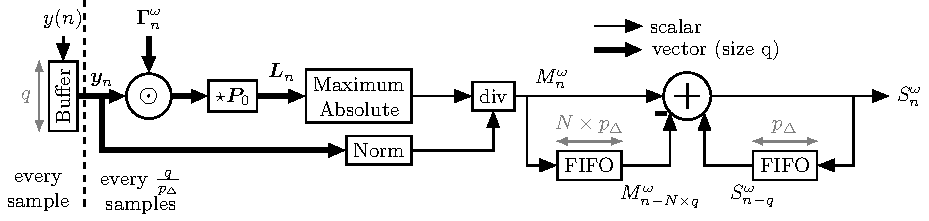
\includegraphics[width=\linewidth]{figures/tikzpicture/score_proc_unit_stdl.pdf}
    \end{column}
    \begin{column}{.5\linewidth}
      \begin{overlayarea}{\linewidth}{.85\textheight}
        \only<1>{
          \includegraphics[width=\linewidth]{figures/pgfplots/score_function_normed.pdf}
        }
        \only<2>{
          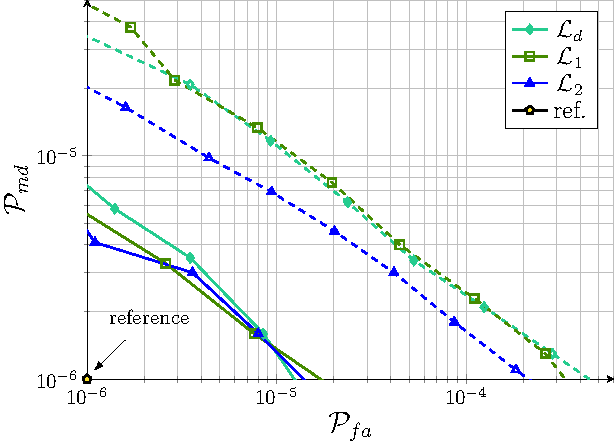
\includegraphics[width=\linewidth]{pgfplots/roc_curves_norms_zoom_stdl.pdf}
          \captionof{figure}{Courbes ROC pour les normes étudiées à un SNR de $-10$ dB, pour $N = 60$ et $q = 64$.}
        }
      \end{overlayarea}
    \end{column}
  \end{columns}
  \footnotetext{Une étude approfondie est disponible dans le manuscrit.}
  \note{
    I - Le score --- II - Impact sur perfo
    \begin{enumerate}
      \item solution que \textbf{J'AI} proposée
      \item bla bla
      \item Etude de complexité et impact que \textbf{J'AI} menée
    \end{enumerate}
  }
\end{frame}



\subsection{Corrélation glissante dans le temps (\emph{Time sliding})}

\begin{frame}{Criticité de la tâche de corrélation}
  \begin{columns}
    \begin{column}{.5\linewidth}
      \begin{overlayarea}{\linewidth}{.33\textheight}
        Le calcul du score est la partie la plus critique du détecteur :
        \begin{itemize}
          \item Débit moyen le plus élevé
          \item Utilisation continue
          \item Forte complexité calculatoire
        \end{itemize}
      \end{overlayarea}
    \end{column}
    \begin{column}{.4\linewidth}
      \begin{overlayarea}{\linewidth}{.2\textheight}
        La corrélation circulaire est la partie la plus complexe de cette tâche critique.
      \end{overlayarea}
    \end{column}
  \end{columns}
  { \centering
  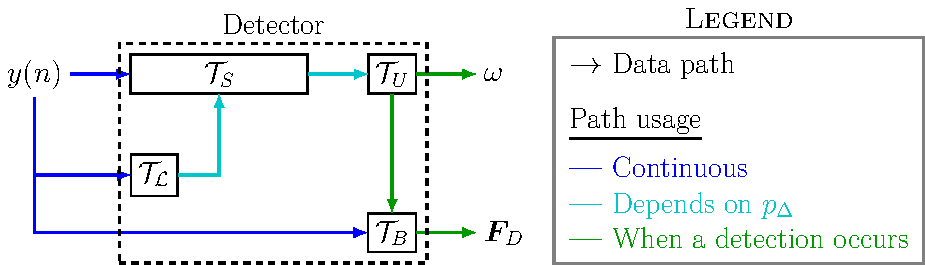
\includegraphics[
    width=\linewidth,
    height=.4\textheight,
    keepaspectratio=true
  ]{figures/tikzpicture/tasks_dep_stdl.pdf}
  \captionof{figure}{$\task{S}$ : calcul de score --- $\task{\mnorm{}}$ : calcul de la norme --- $\task{U}$ : décision --- $\task{B}$ : Tampon mémoire}
  \par}%
  \note{
    \textit{Fais l'point, t'es plus} \textbf{focus} 
    
    Focaliser les efforts.

    \vspace*{2 em}

    \begin{itemize}
      \item Dans le recepteur -> Détection
      \item Dans détecteur -> Score
      \item Dans Score -> Corrélation.
    \end{itemize}
  }
\end{frame}

\begin{frame}{Méthode par transformée de Fourier rapide (FFT)}{}
  \begin{columns}
    \begin{column}{.45\linewidth}
      \begin{overlayarea}{\linewidth}{.55\textheight}
        \only<1>{ \vspace{2 em}

          \centering
          $\vect{L}^{\bomega}_{n} = \mifft{\mfft{\vect{y}_n  \odot \bm{\Gamma}^{\bomega}_n} \odot \mfft{\mpn{0}}^{*}}$ \vspace{1 em}

          $\mfft{\bm{y}}$ : FFT de $\bm{y}$ \\
          $\mifft{\bm{Y}}$ : IFFT de $\bm{Y}$ \\
          $\bm{\Gamma}^{\bomega}_n$ : Vecteur Correcteur de fréquence
        }%
        \only<2>{%
          \centering
          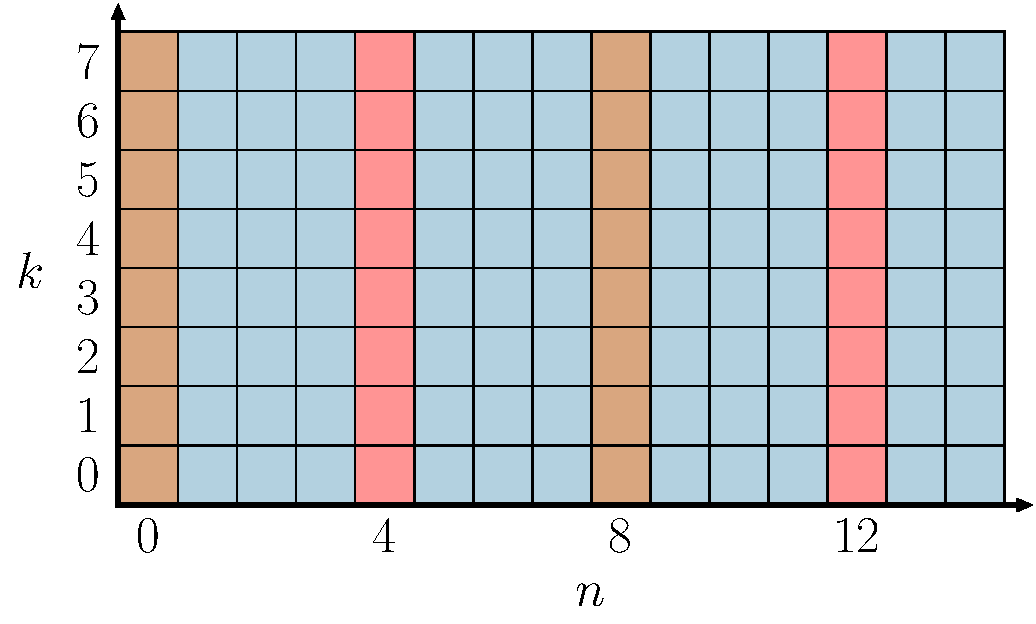
\includegraphics[
            width=\linewidth,
            height=.45\textheight,
            keepaspectratio=true
          ]{figures/tikzpicture/comp_fft_grid_stdl.pdf} \vspace{-1 em}

          \captionof{figure}{Résultat si \textcolor{Red}{$\mpd{} = 2$} pour $q = 8$}
        }%
      \end{overlayarea}
    \end{column}
    \begin{column}{.55\linewidth}
      \centering
      \vspace{-.5 em}
      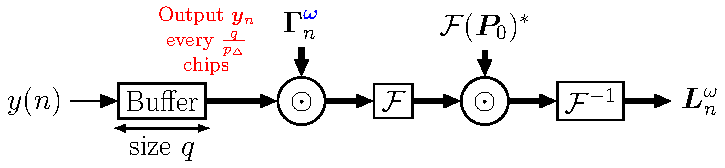
\includegraphics[
        width=\linewidth,
        height=.7\textheight,
        keepaspectratio=true
      ]{figures/tikzpicture/arch_fft_sync_stdl.pdf} \\

      {\scriptsize Complexité pour $1$ corrélation\\ $\sim \mathcal{O}(q^2) \rightarrow \sim \mathcal{O}(q \log_2(q))$}
%       \note{
    \end{column}
  \end{columns}


  \begin{columns}
    \begin{column}{.8\linewidth}
      Méthode dérivant de la démodulation CCSK.
      \begin{ctrlitemize}{0pt}
        \item [\textcolor{Chartreuse4}{$\bm{\oplus}$}] Largement étudiée dans la littérature \cite{abassiNonbinaryLowdensityParitycheck2013,kastnerParallelProgrammingFPGAs2018}.
        \item [\textcolor{Chartreuse4}{$\bm{\oplus}$}] Versatile, duplicable afin de faire varier les paramètres \textcolor{red}{\pd{}} et \textcolor{blue}{\po{}}.
        \item [\textcolor{Red3}{$\bm{\ominus}$}] Peu adapté au traitement d'un flux de données
      \end{ctrlitemize}
    \end{column}
  \end{columns}
  \blfootnote{\textcite{abassiNonbinaryLowdensityParitycheck2013, kastnerParallelProgrammingFPGAs2018}}
  \note{
    \begin{itemize}
      \item Méthode original utilisé dans les travaux de K.S. utilisent des FFT
      \item PK ? Litterature
      \item Pour un calcul -> de $q^2$ à $q\log_2(q)$
      \item si $1$ calcul tous les $4$ ech. ($q = 8$, $\mpd{} = 2$), à $1$ Méch/s -> $250~000$ FFT et IFFT par seconde !
    \end{itemize}
  }
\end{frame}

\begin{frame}{Méthode par \acrfull{ts}}{}
  {%
    \centering
    \includegraphics[
      width=\linewidth,
      height=.24\textheight,
      keepaspectratio=true
    ]{figures/tikzpicture/detect_trame_compare.pdf}\\

    {\scriptsize Complexité pour $1$ corrélation :
    $\sim \mathcal{O}(q \log_2(q)) \rightarrow \sim \mathcal{O}(q)$}
    \par%
  }%
  \begin{columns}
    \begin{column}{.45\linewidth}
      \begin{overlayarea}{\linewidth}{.5\textheight}
        \only<1>{ \vspace{2 em}
        \centering
        $\forall k \in \llbracket 0, \:q - 1 \rrbracket$ \vspace{1 em}

        $L^{\omega}_{n}(k) = L^{\omega}_{n - 1}(k - 1) + P_{k}(q - 1)d_{n}^{\bomega}$,
        \vspace{1 em}

        {\small $d_{n}^{\bomega} = [y(n)\Gamma^{\bomega}(n)] - [y(n - q)\Gamma^{\bomega}(n - q)]$}

        }%
        \only<2>{%
          \centering
          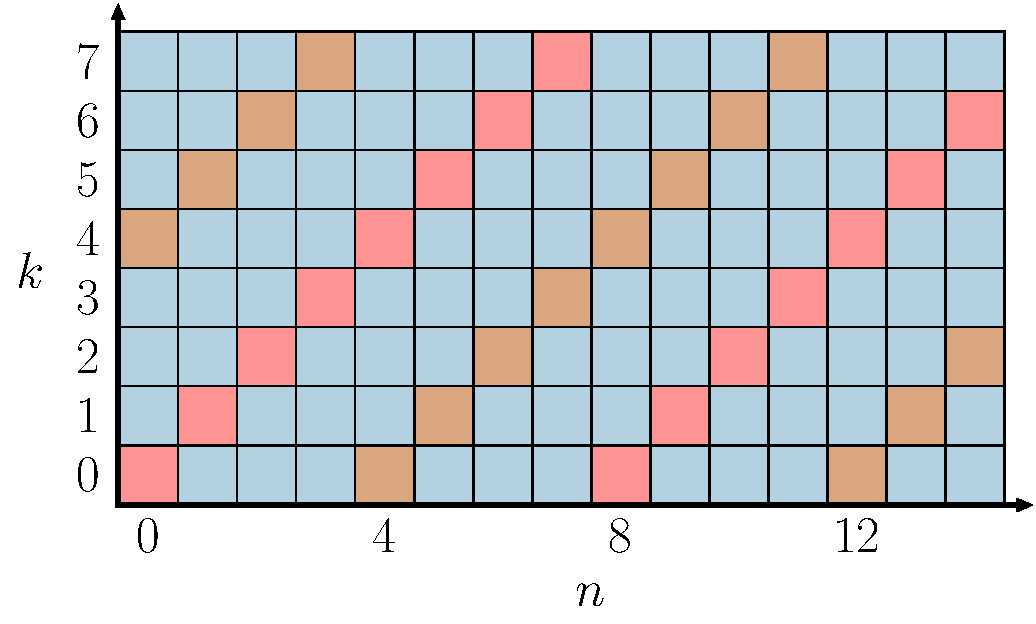
\includegraphics[
            width=\linewidth,
            height=.45\textheight,
            keepaspectratio=true
          ]{figures/tikzpicture/comp_ts_grid_stdl.pdf} \vspace{-1 em}

          \captionof{figure}{Résultat si \textcolor{Red}{$\mpd{} = 2$} pour $q = 8$}
        }%
        
      \end{overlayarea}
    \end{column}
    \begin{column}{.55\linewidth}
      Nouvelle méthode, mise au point spécialement pour la détection QCSP.
      \begin{ctrlitemize}{0pt}
        \item [\bonus] Moins complexe que la méthode par \fft{} quand \textcolor{red}{$\mpd{} > \frac{q}{\log_2(q)}$} \cite{moniereTimeSlidingWindow2021}\\$\Rightarrow$ $\nearrow$ efficience.
        \item [\malus] Le degré de liberté sur \textcolor{red}{\pd{}} est perdu.
      \end{ctrlitemize}
    \end{column}
  \end{columns}
  \blfootnote{\textcite{moniereTimeSlidingWindow2021}}
  \note{
    \begin{itemize}
      \item Nouvelle méthode que \textbf{NOUS} avons mise au point
      \item PK ? dans le temps, adapté à un flux de données par conception
      \item MAIS besoin de tous les points !!
      \item Pour un calcul -> de $q\log_2(q)$ à $q$ et \pd{} is $q$
      \item si \pd{} $>$ \dots OK
    \end{itemize}
  }
\end{frame}

\begin{frame}{Deux versions : \textit{data shift} et \textit{index shift}}{}
  \centering
  \begin{tikzpicture}[overlay, remember picture]
    \node at ($(current page.north) + (-.1, -2.5)$) {%
      \includegraphics[
        width=\linewidth,
        height = .19\textheight,
        keepaspectratio = true]{figures/tikzpicture/arch_ts_dnw.pdf}
    };
  \end{tikzpicture}

  \vspace{-1 em}
  \begin{columns}
    \begin{column}{.5\linewidth}
      \begin{overlayarea}{\linewidth}{.9\textheight}
        \centering
        \includegraphics[width=\linewidth, height=.5\textheight, keepaspectratio=true]{figures/tikzpicture/arch_statts_sync_corr.pdf}
        \captionof{figure}{Corrélation partielle ``\emph{data shift}''}
        % \vspace{-1 em}

        \begin{ctrlitemize}{0pt}
          \item [\bonus] Intuitive, sortie ordonnée.
          \item [\malus] Lourde, les $L^{\bomega}_{n}(i)$ sont des nombres complexes, et toujours représentés sur plusieurs bits.
        \end{ctrlitemize}
      \end{overlayarea}
    \end{column}
    \begin{column}{.5\linewidth}
      \begin{overlayarea}{\linewidth}{.9\textheight}
        \centering
        \includegraphics[width=\linewidth, height=.5\textheight, keepaspectratio=true]{figures/tikzpicture/arch_subts_sync_corr.pdf}
        \captionof{figure}{Corrélation partielle ``\emph{index shift}''}
        % \vspace{-1 em}

        \begin{ctrlitemize}{0pt}
          \item [\bonus] Légère, les $P_{k + i}(q - 1)$ sont des nombres réels, pouvant être représentés par $1$ bit.
          \item [\textcolor{RoyalBlue}{\malus}] Sortie désordonnée, mais \dots{} l'ordre n'importe pas \textit{en détection}.
        \end{ctrlitemize}
      \end{overlayarea}
    \end{column}
  \end{columns}
\end{frame}

\begin{frame}
  \frametitle{Algorithme de détection efficace}
  \begin{columns}
    \begin{column}{.5\linewidth}
      \begin{ctrlitemize}{.5 em}
        \item Algorithme robuste à des variations de gain d'entrée ;
        \item Nouvelle méthode de corrélation plus efficace\footnotemark.
      \end{ctrlitemize} \vspace{1 em}

      \begin{ctrlitemize}{.5 em}
        \item Insuffisant pour atteindre un débit temps réel ;
        \item Le débit d'information ``algorithmique'' du système atteint $5$ kb/s, $10\times$ moins que le LoRa \dots
      \end{ctrlitemize}
    \end{column}
    \begin{column}{.4\linewidth}
      \centering
      \includegraphics[width = \linewidth]{figures/pgfplots/results_algo_through.pdf}
      \captionof{figure}{Débits logiciels en l'absence d'optimisation sur serveur Intel\textregistered{} Xeon\texttrademark{}, horloge $3.0$ GHz.}
    \end{column}
  \end{columns} \vspace{-1 em}
  \footnotetext{Meilleur rapport performances de détection / complexité calculatoire.}
\end{frame}

\end{document}
